\documentclass[tikz,border=3mm]{standalone}
\usetikzlibrary{matrix,positioning,fit,backgrounds}
\begin{document}
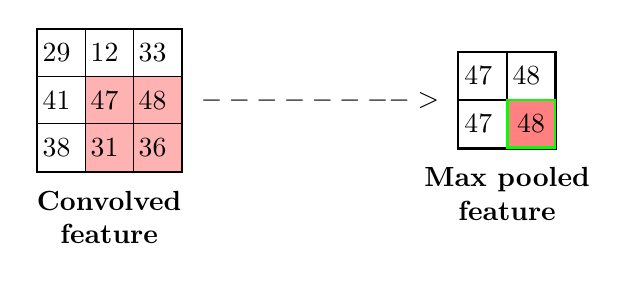
\begin{tikzpicture}[mmat/.style={matrix of nodes,
	column sep=-\pgflinewidth/2,
   row sep=-\pgflinewidth/2,
   cells={nodes={draw,inner sep=2pt,thin}},draw=#1,thick,inner sep=0pt},
  nodes in empty cells,
  nodes={
  	minimum size=.6cm,
  	anchor=center,
  	align=center,
  	},
   mmat/.default=black,
   node distance=0.3em]
 
 \matrix[mmat](mat1){    
     29  & 12 & 33 \\ 
      41 & 47 & 48 \\
      38 & 31 & 36 \\ 
     };
 \node [below= of mat1.south] (f) {\bf Convolved \\ \bf feature};
 \node[right=of mat1](eq){$-------->$} ; 
 \scoped[on background layer]
 {
 	\node[fill=red!30, fit=(mat1-2-2)(mat1-3-3),inner sep=0pt] {};
 }
 \matrix[mmat, right=of eq](mat2){    
 	47  &  48 \\ 
 	 47 &   |[draw=green, thick, fill=red!50]|48\\
 	};
\node [below = of mat2.south] {\bf Max pooled \\ \bf feature};

\end{tikzpicture}
\end{document}
